\section{Background}\label{sec-background}
In this section, we briefly overview our prior work and the new challenges in the MV setting.

%\begin{figure}[t] 
%\centering
%\vspace{-0.75em}
% 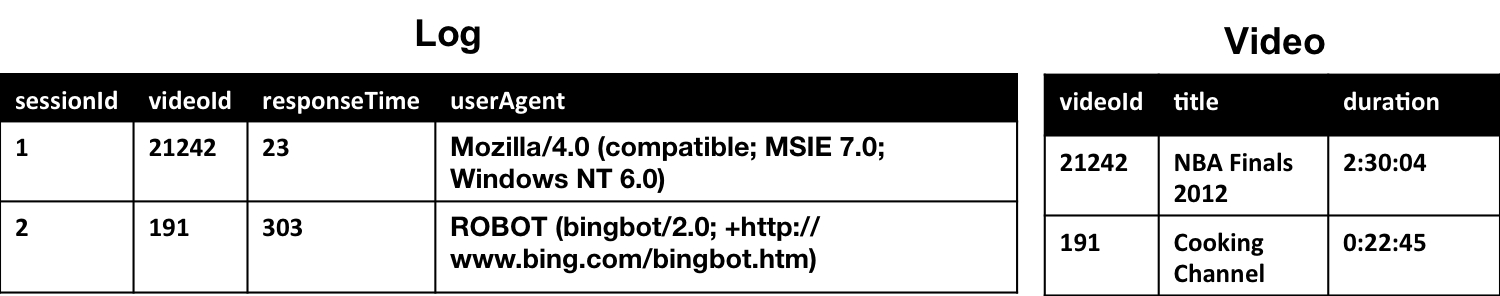
\includegraphics[width=\columnwidth]{figs/sample-clean-example.png}\vspace{-0.25em}
% \caption{A simplified log analysis example dataset. In this dataset, there are two tables: a fact table representing video views and a dimension table representing the videos.\label{example-1}}\vspace{-1em}
%\end{figure}

\iffalse
\subsection{Materialized View Maintenance}\label{subsec-inc}
Views define logical relations which can be queried instead of physical base relations.
MVs are a class of views that are pre-computed and stored (i.e materialized).
Any form of pre-computed, derived data encounters the problem of staleness when the physical base relations update.

One approach to this problem is to recompute the materialized view every time there are updates to the base tables.
However, this approach is very inefficient if updates to the data generally have small or sparse effect on the MV. 
A contrasting approach is incremental view maintenance (IVM), where rows in the MV are incrementally updated based on the updates to the base table.
Incremental maintenance of MVs has been well studied; see \cite{chirkova2011materialized} for a survey of the approaches. 
At a high-level, incremental maintenance algorithms typically consist of the following steps: (1) maintain a cache of insertions and deletions for each physical base table, then using the view definition derive a \emph{change propagation formula} in terms of the set of insertions and deletions, and finally apply the formula to the view.
For a variety of view types, these rules are described in detail in \cite{DBLP:journals/vldb/KochAKNNLS14, DBLP:conf/pods/Koch10}.

%Incremental maintenance may not be efficient in all cases.
%Consider the view that calculates the median \tbl{responseTime} grouped by \tbl{userAgent} on our running example dataset.
%In general, to ensure correctness, the view has to store the entire set of \tbl{responseTime} attributes for each group to allow for incremental maintenance.
%Along the lines of this example, there are cases when recomputation may require less storage of state or even less computation.
%Thus, materialized views are maintained either with incremental maintenance, recomputation, or a mix.

In real-world systems, for large datasets or fast data update rate, it may not always be feasible to maintain MVs immediately. 
Therefore, deferring maintenance (periodically or adaptively) is an alternative and often preferred solution.
The main insight of deferral is to avoid maintaining the view immediately and to schedule an update at a more convenient time.
In deferred maintenance approaches, the user often accepts some degree of staleness for additional flexibility in scheduling.
%\svc offers a data cleaning perspective on this problem, namely, there is a trade-off between the query result accuracy and computation.
By using sampling, we give the user access to a new trade-off space between immediate (or close to immediate, i.e., mini-batch) maintenance and long-periodic maintenance.

%In particular, we highlight a technique called lazy maintenance which applies updates to the view only when a user's query requires a row \cite{zhou2007lazy}.
%While always fresh, both lazy maintenance and immediate maintenance hit a bottleneck when there are rapid updates, and this results increasingly degraded performance if a user wants to query a view.
%The alternative is a periodic strategy, but this means that there is unbounded error on queries between maintenance periods.
%\subsubsection{Practical Considerations}
\fi


\subsection{SampleClean~\cite{wang1999sample}}
SampleClean is a framework for scalable aggregate query processing on dirty data.
Traditionally, data cleaning has explored expensive, up-front cleaning of entire datasets for increased query accuracy, and those who were unwilling to pay the full cleaning cost avoided data cleaning altogether.
We proposed SampleClean to add an additional trade-off to this design space by using sampling.
This challenge mirrors the challenge face \reminder{faced?} in the MV setting with the tradeoff between immediate maintenance (inexpensive and inaccurate) and deferred maintenance (expensive and accurate).

SampleClean has three parts: (1) sampling, (2) data cleaning, and (3) query result estimation.
First, SampleClean creates a sample of dirty data (which may have erroneous values or duplicated records). %(which are erroneous, missing, or otherwise corrupted records).
Then, the framework applies a data cleaning procedure to the sample.
Finally, when users query the dataset, the framework uses the cleaned sample to extrapolate clean query results.
In the framework, the main challenge was that data cleaning can potentially change the statistics of a sample and the queries need to compensate for those effects.
%In our initial work, SampleClean mainly focused on three common aggregates: \sumfunc, \avgfunc, and \countfunc queries.

The SampleClean work showed that there were two contrasting approaches to query processing on a sample of cleaned data.
We could (1) clean the sample first and then run the query on the sample, or (2) look at the difference between the clean and dirty samples and calculate a correction to correct an existing dirty query result. 
Approach (1) is similar to those studied in the Approximate Query Processing (AQP) literature \cite{OlkenR86,AgarwalMPMMS13, joshi2008materialized}.
Approach (2), which we called \nsc, outperformed (1) in datasets where data error was small or sparse.
In the MV setting, we compare these approaches (see Section \ref{exp}). 

%\begin{figure}[t] \vspace{-2em}
%\centering
% 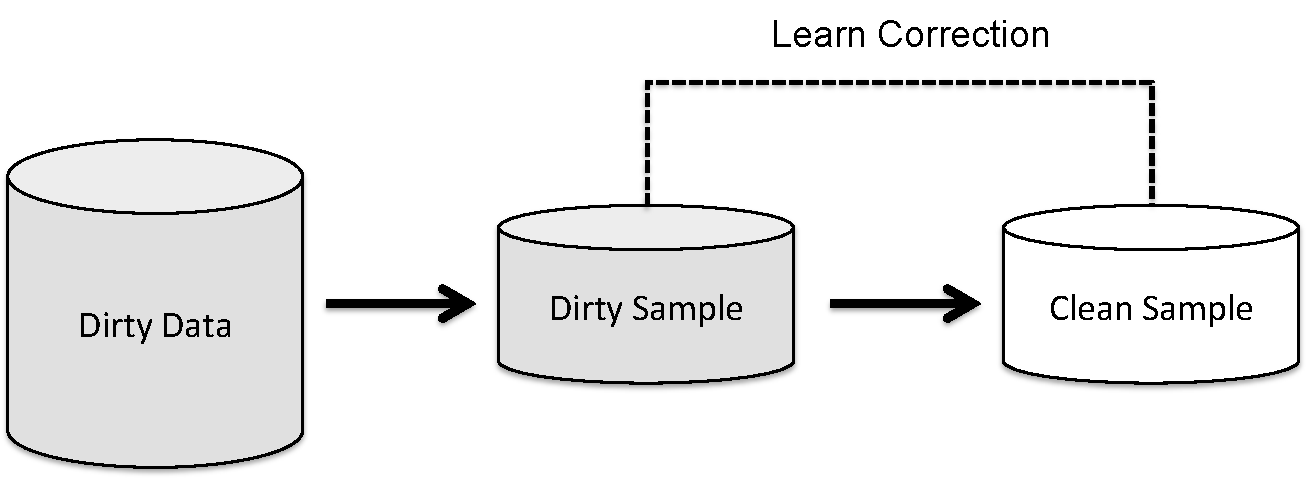
\includegraphics[scale=0.26]{figs/sys-arch2.pdf} \vspace{-.25em}
% \caption{A basic overview of SampleClean. SampleClean uses a random sample of dirty data to learn how a data cleaning algorithm affects queries on the sample. We can then derive a correction to compensate for the dirtiness.\label{sc}}\vspace{-1.75em}
%\end{figure}

\subsection{New Challenges}
%Applying SampleClean to materialized maintenance requries significant extensions to both the data cleaning, and query processing.
The consequence of staleness is data error and then view maintenance can be posed as the data cleaning as it removes these errors.
But note that we cannot simply extend SampleClean to MVs, and there are many significant new challenges that we have to address.

The first challenge is about data cleaning. In SampleClean, we modeled data cleaning as a row-by-row transformation of table. 
This transformation was a user-specified  ``black box'' that operated on each row, and we applied this to a sample of dirty data.
%The consequence of staleness is data error and then view maintenance can be posed as the data cleaning as it removes these errors.
However, in a MV setting, we found that the ``black-box'' data cleaning model does not suffice.
First, applying incremental maintenance to a sample may not be any more efficient than applying it to a whole MV if it does unnecessary computation.
In this work, we analyze the relational algebra of a MV maintenance procedure and propose a series of rules to optimize maintaining a sample.
Second, stale MVs have not only incorrect rows, but also rows that are missing from the ``dirty'' view or conversely need to be deleted. We need to define a new data-cleaning model to handle this type of error. 
%When coupled with sampling, this poses significant challenges since the statistics of the ``dirty'' (stale) sample are different from the ``clean'' (up-to-date) sample. \reminder{I did not get this point. Does SampleClean have the same issue?}
%We address this problem by formalizing the necessary updates to a sample materialized view as a data cleaning procedure.
%There is further a new challenge in how to most efficiently execute this procedure to avoid irrelevant computation. 

%This requires us to significantly extend SampleClean in terms of query processing.
%In SampleClean, \nsc calculated the difference between the ``dirty'' and the ``clean'' sample, we extend this approach to settings where those samples do not match perfectly due to missing data.
In terms of supported queries, SampleClean mainly focused on three common aggregates: \sumfunc, \avgfunc, and \countfunc queries.
In this work, we explore a broader set of aggregate queries such as \medfunc and design a bootstrap algorithm to bound the approximation error.
We found that the queries that we studied before (\sumfunc, \avgfunc, and \countfunc) were actually a special case where our estimates are optimal.

Sampling is particularly sensitive to variance of the dataset, and large outliers can significantly reduce query accuracy, so in this work, we extend the query processing with an index of outliers.
However, in this setting, an important challenge is to efficiently compute the outlier index.
We show that with only a single pass of the base data, we can index records that exceed some threshold.
Then, for all rows in an MV that are dependent on an indexed record, we can ensure that they are included in our sample MV.
We found that empirically this approach lead\reminder{led?} to significant accuracy improvements in skewed datasets.

\subsection{Running Example: Server Log Analysis}
To illustrate our framework in the upcoming sections, we use the following running example which is a 
simplified schema of one of our experimental datasets.
%(Figure~\ref{example-1}).
Imagine, we are querying logs from a video streaming company. 
These logs record visits from users as they happen and grow over time.
We have two tables, \tbl{Log} and \tbl{Video}, with the following schema:
\begin{lstlisting}[mathescape,basicstyle={\scriptsize}]
Log(sessionId$\textrm{,}$ videoId$\textrm{,}$ responseTime$\textrm{,}$ userAgent)
Video(videoId$\textrm{,}$ title$\textrm{,}$ duration)
\end{lstlisting}
The \tbl{Log} table stores each visit to a specific video with primary key (\textsf{sessionId}), a foreign-key to the \tbl{Video} table (\textsf{videoId}), latency of the visit (\textsf{responseTime}), and the browser used to access the video (\textsf{userAgent}).
The \tbl{Video} stores each video with the primary key (\textsf{videoId}), the video title (\textsf{title}), and the video duration (\textsf{duration}).
Though \svc supports insertions, deletions, and updates to base data (See Section~\ref{notation} for details), for clarity in our example, we consider insertions
into Log which is cached in a temporary table:
%\reminder{I replace LogInserts with LogIns for saving a line of space. Make sure it is consistent in the whole paper.}
\begin{lstlisting}[mathescape,basicstyle={\scriptsize}]
LogIns(sessionId$\textrm{,}$ videoId$\textrm{,}$ responseTime$\textrm{,}$ userAgent)
\end{lstlisting}




